\chapter{Results}
\label{chap:results}

\begin{figure}[H]
\centering
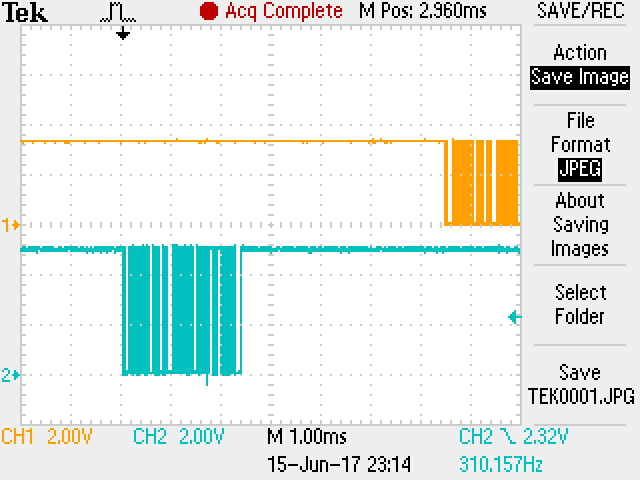
\includegraphics[width=0.8\textwidth]{Figures/delay_tx_rx.JPG}
\caption{Delay in TX an RX}
\label{fig:delay_tx_rx}
\end{figure}


Figure~\ref{fig:delay_tx_rx} shows the TX signal of the transmitting module (Blue) and the RX signal of the receiving module (Yellow).
The delay between transmitting a package and receiving the package at the other module is \SI{6.5}{\milli\second}.
Due this delay there is a difference of \SI{6.5}{\milli\second} between the measured TDOA and the actual $\Delta t$ (see figure~\ref{fig:ultra1}) as discussed in section~\ref{sec:delay}.
This means the distance calculated using the measured $\Delta t$ is:

$ v_{sound} * t_{delay} = \SI{340.29}{\meter\per\second} * \SI{6.5}{\milli\second} = \SI{2.2}{\meter} $

lower than the actual distance between the modules.
The distance corresponding to the delay, \SI{2.2}{\meter}, will be added the to result of the distance measuring test to show that the measurements are correct when the delay is taken into account.
At this point this has to be done manually but in the future a method to deal with this delay will be implemented as discussed in section~\ref{sec:delay}.

When we perform the measurement of the delay between TX and RX multiple times with different distances between the two modules we notice the following:

\begin{itemize}
\item
The delay is independent of the distance between transmitter and receiver.
\item
The delay varies with time.
It has an average of \SI{6.5}{\milli\second} and a deviation of \SI{0.5}{\milli\second}.
So the delay lies anywhere between \SI{6}{\milli\second} and \SI{7}{\milli\second}.
\end{itemize}

This means that, by using the average delay to compensate for the effect of the delay, a maximum error of $\pm$ \SI{0.5}{\milli\second} is introduced to $\Delta t$.
This error corresponds to a distance error of:

$ v_{sound} * \pm t_{error} = \SI{340.29}{\meter\per\second} * \pm \SI{.5}{\milli\second} =\pm \SI{17}{\centi\meter} $


\begin{figure}[H]
\centering
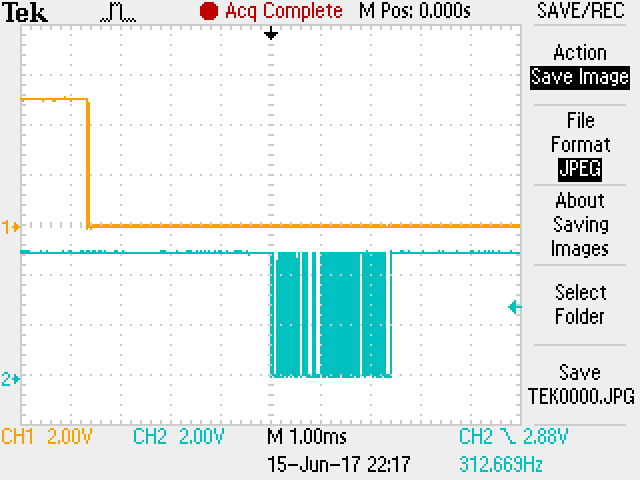
\includegraphics[width=0.8\textwidth]{Figures/test_1m.JPG}
\caption{Measurement with a distance of \SI{1}{\meter} between modules}
\label{fig:mes_1}
\end{figure}

Figure~\ref{fig:mes_1} shows the $US_{detect}$ signal (Yellow) and the RX signal (Blue) of a single module.
The falling edge in the $US_{detect}$ signal is the time at which a ultrasonic pulse is first detected.
Since the distance between the modules is smaller than the distance corresponding to the delay, the ultrasonic pulse arrives at the module before the start package of the RF message.
The TDOA between the ultrasonic pulse and the start of the RF message is \SI{3.6}{\milli\second}.
Since the RF message is transmitted \SI{6.5}{\milli\second} after the ultrasonic pulse $\Delta t$ can be calculated by, in this case, by subtracting the measured TDOA from the delay.
This gives a $\Delta t$ of:

$ \Delta t = t_{delay} - TDOA = \SI{6.5}{\milli\second} - \SI{3.6}{\milli\second} = \SI{2.9}{\milli\second} $

Which corresponds to a distance of:

$ v_{sound} * t_{delay} = \SI{340.29}{\meter\per\second} * \SI{2.9}{\milli\second} = \SI{1}{\meter} $

Although the resolution of the measurement is low since the TDOA is estimated with the oscilloscope (to one decimal) it shows that the distance measurements are correct when the delay is taken into account.
In the fully integrated prototype these TDOA measurements will be done with a microcontroller resulting in a higher resolution.
Unfortunately this hardware is not available at the point of writing so it's impossible to make conclusions on the accuracy of the measurement.

\begin{figure}[H]
\centering
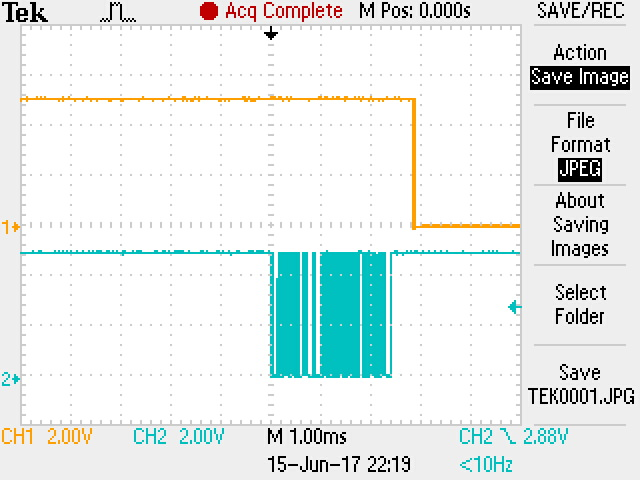
\includegraphics[width=0.8\textwidth]{Figures/test_3m.JPG}
\caption{Measurement with a distance of \SI{3}{\meter} between modules}
\label{fig:mes_3}
\end{figure}


Figure~\ref{fig:mes_3} shows the $US_{detect}$ signal (Yellow) and the RX signal (Blue) of a single module for the second measurement done for a distance of \SI{3}{\meter}.
In this case the distance is larger than the distance corresponding to the delay so the ultrasonic pulse arrives after the RF message.
The TDOA between the start of the RF message and the ultrasonic pulse is \SI{2.8}{\milli\second}.
Since the RF message is transmitted \SI{6.5}{\milli\second} after the ultrasonic pulse $\Delta t$ can be calculated by, in this case, adding the delay to the measured TDAO.
This gives a $\Delta t$ of:

$ \Delta t = TDOA + t_{delay}  = \SI{2.8}{\milli\second} + \SI{6.5}{\milli\second} = \SI{9.3}{\milli\second} $

Which corresponds to a distance of:

$ v_{sound} * t_{delay} = \SI{340.29}{\meter\per\second} * \SI{9.3}{\milli\second} = \SI{3.2}{\meter} $

\begin{figure}[H]
\centering
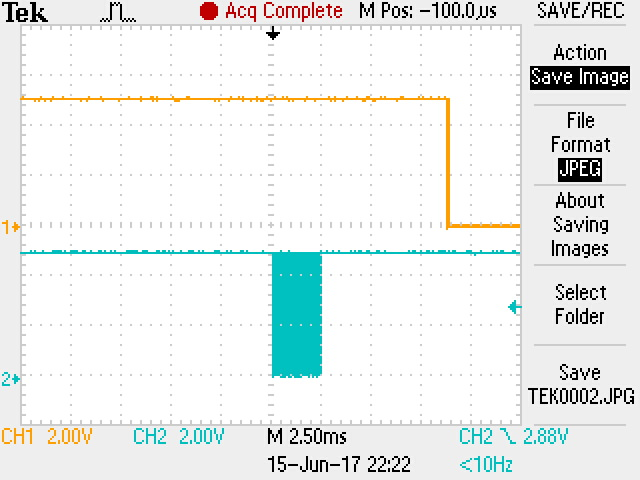
\includegraphics[width=0.8\textwidth]{Figures/test_5m.JPG}
\caption{Measurement with a distance of \SI{5}{\meter} between modules}
\label{fig:mes_5}
\end{figure}

Figure~\ref{fig:mes_5} shows the $US_{detect}$ signal (Yellow) and the RX signal (Blue) of a single module for the third measurement done for a distance of \SI{5}{\meter}.
Note that the scale is different than the first two measurements.
The TDOA between the start of the RF message and the ultrasonic pulse is \SI{8.8}{\milli\second}.
Since the RF message is transmitted \SI{6.5}{\milli\second} after the ultrasonic pulse $\Delta t$ can be calculated by, in this case, adding the delay to the measured TDAO.
This gives a $\Delta t$ of:

$ \Delta t = TDOA + t_{delay}  = \SI{8.8}{\milli\second} + \SI{6.5}{\milli\second} = \SI{15.3}{\milli\second} $

Which corresponds to a distance of:

$ v_{sound} * t_{delay} = \SI{340.29}{\meter\per\second} * \SI{15.3}{\milli\second} = \SI{5.2}{\meter} $

\section{Results after integration}

This section shows the results acquired after the initial deadline of the Thesis.
Before the deadline it was not yet possible to do these measurements since the distance sensing system was not yet integrated with the microcontroller.
For each results (plot) we will discuss the test set-up and the conclusions we can draw from these results.
In a separate section in chapter~\ref{chap:conc} the final conclusions after integration will be discussed.

For these measurements a countermeasure for the delay between TX and RX (discussed above) was implemented:
The ultrasonic delay is transmitted \SI{8}{\milli\second} after the RF message.
At the receiving side this \SI{8}{\milli\second} delay is compensated.

For the first measurement (see figure~\ref{fig:int_meas_1}) 2 modules are used.
They are placed a certain distance apart.
We start at \SI{1}{\meter} and increase the distance with \SI{1}{\meter} up to a distance of \SI{6}{\meter}.
At each distance a set of multiple measurements is performed.
To measure the distance between the devices we measure the number of clock cycles between the arrival of the RF signal and the arrival of the US pulse.
The results are given in figure~\ref{fig:int_meas_1}

\begin{figure}[H]
\centering
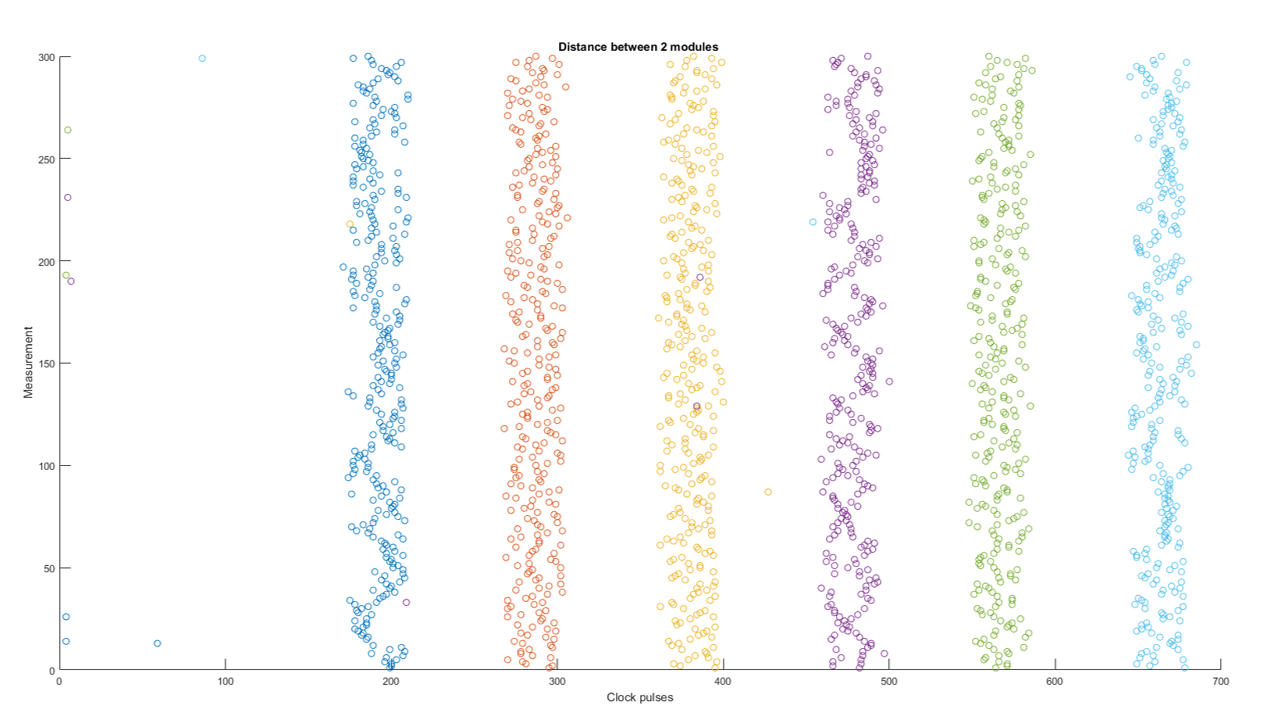
\includegraphics[width=0.9\textwidth]{Figures/Distance_6.png}
\caption{Measurement with static distances: \SI{1}{\meter},\SI{2}{\meter},\SI{3}{\meter},\SI{4}{\meter},\SI{5}{\meter} and \SI{6}{\meter}}
\label{fig:int_meas_1}
\end{figure}

There is a clear visible distinction between the measurements corresponding to the different distances in figure~\ref{fig:int_meas_1}.
Furthermore the spacing between the ``bands'' seems to be constant suggesting a linear relation between the measured number of clock cycles and the distances.
To further analyse the results the measurements of figure~\ref{fig:int_meas_1} are given as boxplots in figure~\ref{fig:int_meas_2}

\begin{figure}[H]
\centering
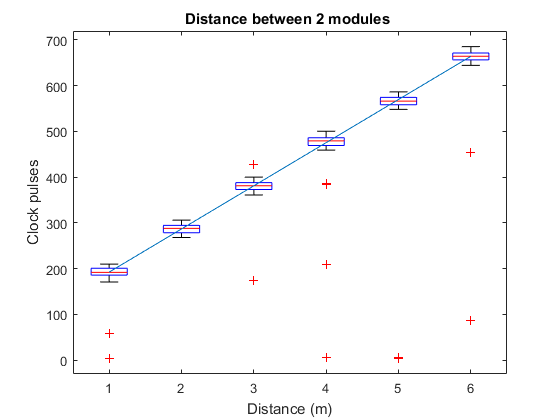
\includegraphics[width=0.8\textwidth]{Figures/Meas_1.png}
\caption{Boxplot representation of static measurements}
\label{fig:int_meas_2}
\end{figure}

From figure~\ref{fig:int_meas_2} the following conclusions are drawn:

\begin{itemize}
\item The relation between the measured number of clock cycles and the distances is linear as can be seen from the fitted line.
\item There are outliers but the differ a lot from mean of the measurements. We thus concludes that these can be easily rejected or filtered.
\item The error (deviation from mean) is constant for all distances. The error does not increase with a greater distance.
\item The error is roughly \SI{20}{\centi\meter} from the mean.
\end{itemize}

We thus draw the conclusion that the integrated system is capable of doing distance measurement between static modules.
With the next test the effect of multiple modules and moving modules is analysed.
Two modules are placed at static locations while the third is placed on a moving skateboard.
The resulting measurements are given in figure~\ref{fig:int_meas_3}.
Module 0 and Module 2 are the static modules, which is clearly visible in figure~\ref{fig:int_meas_3}.
Module 1 is the moving module as in figure~\ref{fig:int_meas_moving}.
In figure~\ref{fig:int_meas_3} this movement is clearly visible:

\begin{itemize}
\item First module 1 moves closer to module 0.
\item It then moves away farther from module 0.
\item Module 1 then moves closer to module 2.
\end{itemize}

This corresponds to the behaviour we expect with the set-up in figure~\ref{fig:int_meas_moving}.
We thus concludes that the systems works with multiple and moving modules.

\begin{figure}[H]
\centering
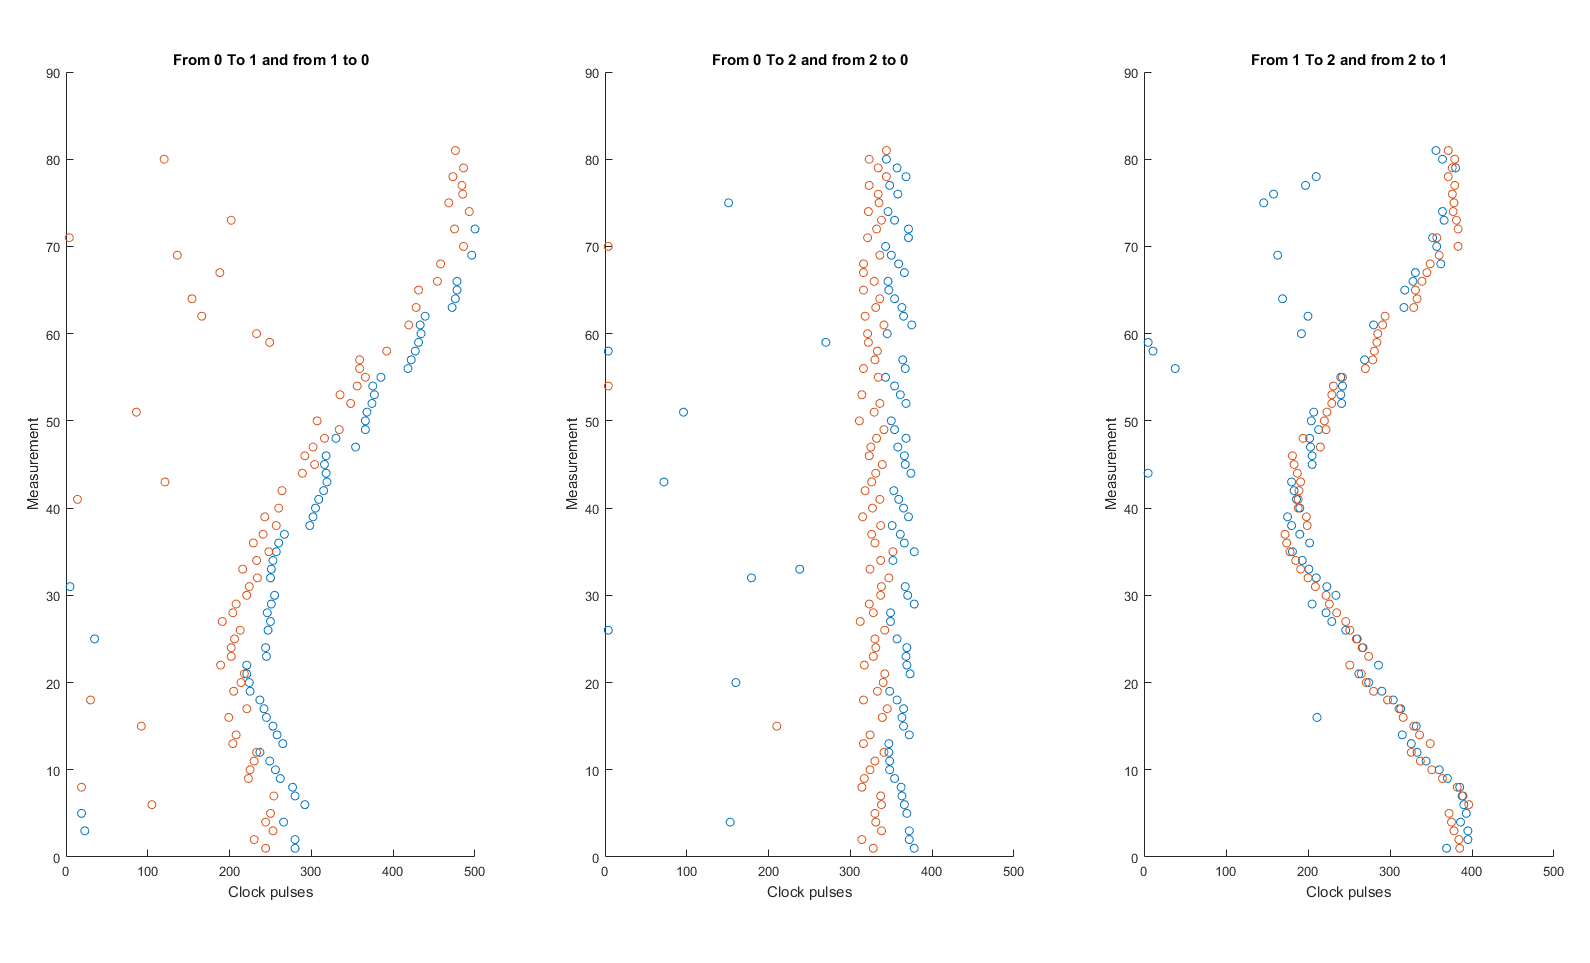
\includegraphics[width=0.9\textwidth]{Figures/meas_skate.png}
\caption{Measurements of moving modules}
\label{fig:int_meas_3}
\end{figure}

\begin{figure}[H]
\centering
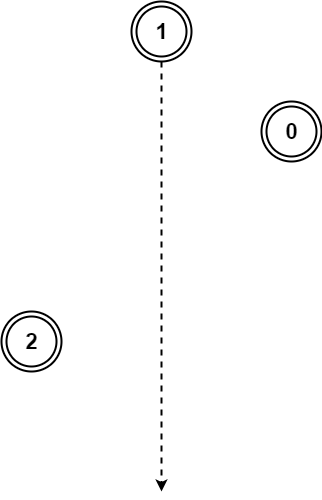
\includegraphics[width=0.4\textwidth]{Figures/moving_module.png}
\caption{Measurement set-up with moving module}
\label{fig:int_meas_moving}
\end{figure}
